% !TEX encoding = UTF-8
% !TEX program = pdflatex
% !TEX root = MEMOC.tex
% !TEX spellcheck = it-IT

\chapter{Laboratorio 1}

\section{Introduzione}

Come solver per i nostri modelli utilizzeremo CPLEX.

Un solver è un'applicazione che prende in input la descrizione di un modello relativo ad un problema di ottimizzazione e fornisce in output una soluzione ottima del problema.

\begin{figure}[htbp]
	\centering
	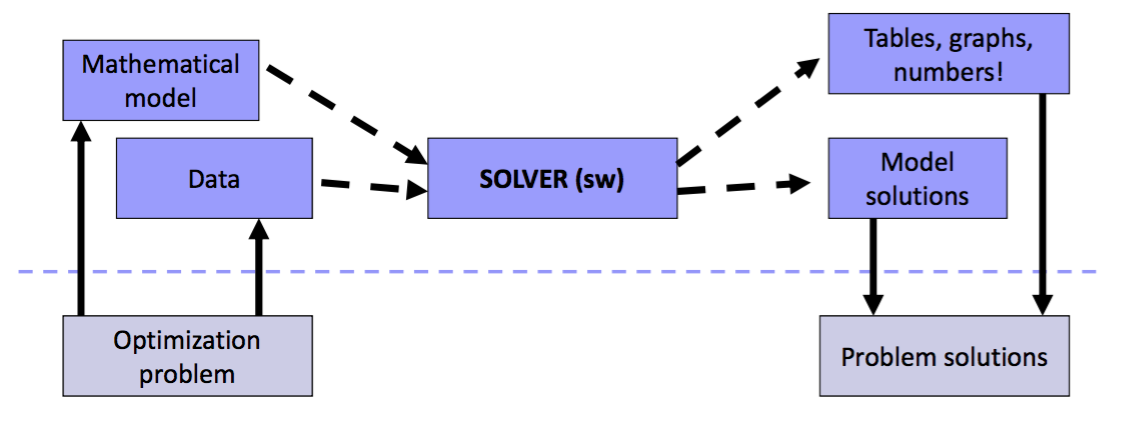
\includegraphics[width=0.7\linewidth]{./images/lab1-schema-1}
\end{figure}

Ovviamente il modello deve essere espresso in una particolare sintassi.

CPLEX è un solver MILP, ovvero un solver in grado di risolvere problemi di programmazione lineare intera mista.
Questa tipologia di solver è quella più comune perché è molto efficiente, non soffre di problemi legati alla stabilità numerica e risulta facilmente embeddabile in altri programmi.

Come anticipato, ogni solver ha una sua interfaccia che può essere utilizzata da dei linguaggi special-purpose o general-purpose.

\begin{figure}[htbp]
	\centering
	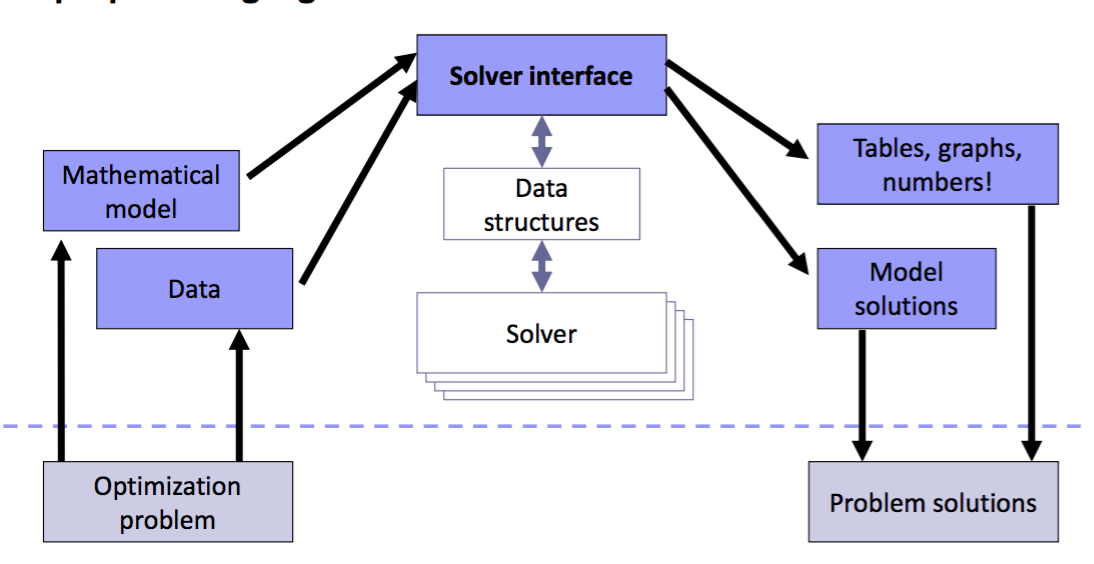
\includegraphics[width=0.7\linewidth]{./images/lab1-schema-2}
\end{figure}

\section{Introduzione a CPLEX}

CPLEX è stato uno dei primi solver e al momento è tra i migliori, in quanto include lo stato dell'arte delle varie tecnologie.

Ci sono varie interfacce utilizzabili per i vari linguaggi di programmazione più diffusi e anche per i linguaggi special-purpose come AMPL. Noi utilizzeremo le API C/C++.

Le \textbf{CPLEX Callable Libraries} implementano varie algoritmi di risoluzione, noi utilizzeremo il MIP, e sono composte da due oggetti principali: \texttt{Environment} e \texttt{Problem}.

\begin{itemize}
	\item \texttt{Enviroment}: contiene le informazioni relative ai parametri di ottimizzazione, alla configurazione, ecc.
	\item \texttt{Problem}: contiene le informazioni di un particolare problema, come i vincoli e le variabili.
\end{itemize}

\noindent\`E necessario che venga definito almeno un \texttt{Environment} e un \texttt{Problem}.

\begin{verbatim}
CPXENVptr CPXopenCPLEX / CPLcloseCPLEX
CPXLPptr CPLcreateprob / CPXfreeprob
\end{verbatim}

\noindent Per interagire con gli oggetti vengono usate le apposite API che seguono più o meno lo stesso schema

\begin{verbatim}
int CPXfuncName (eviroment[,problem],...);
\end{verbatim}

\noindent L'intero ritornato è un codice errore, se è 0 vuol dire che l'operazione è andata a buon fine.

\section{Rappresentazione con matrici sparse}

Un modello generico può essere rappresentato da delle matrici:

\begin{align*}
\min/\max & C^T x \\
\st & A x = b \\
	& x \geq 0
\end{align*}

\noindent con $x,C \in \mathbb{R}^n$, $A \in \mathbb{R}^{m \times n}$ e $b \in \mathbb{R}^m$.

Nei casi reali la matrice $A$ risulta essere molto grande e sparsa, ovvero con molti elementi uguali a 0.

Questa matrice viene quindi rappresentata con 3 vettori:

\begin{itemize}
	\item \texttt{double* val}: contiene i valori della matrice in modo compatto (uno dietro l'altro).
	\item \texttt{int* idx}: contiene l'indice della colonna del valore che si trova alla stessa posizione del vettore \texttt{val}. La lunghezza di \texttt{idx} è la stessa di \texttt{val}.
	\item \texttt{int* beg}: contiene gli indici per il vettore \texttt{val} dove iniziano le righe della matrice.
\end{itemize}

\begin{figure}[htbp]
	\centering
	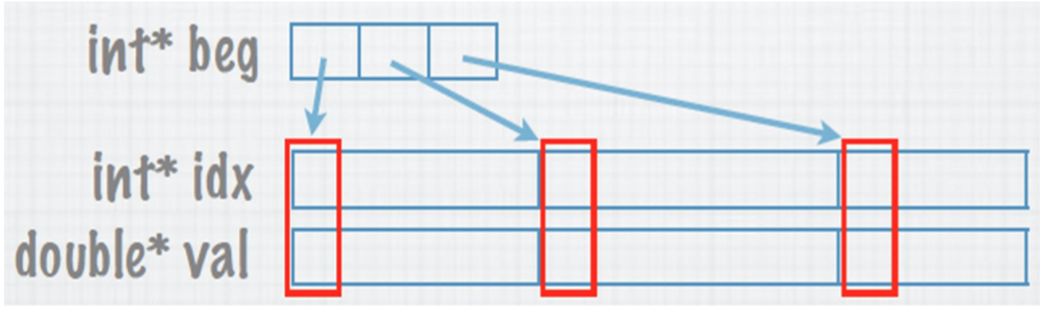
\includegraphics[width=0.5\linewidth]{./images/lab1-matrix}
\end{figure}

\section{Utilizzo di CPLEX}

Per avviare l'ambienti di CPLEX nel terminale è necessario eseguire i comandi:

\begin{verbatim}
$ . clpex_env
$ cplex
\end{verbatim}

\noindent Nel file \texttt{02.firstModel/cpxmacro.h} ci sono delle macro che facilitano la creazione dell'ambiente e del problema.
Abbiamo pure un makefile che compila tutto, che bello!